\item \textbf{{[}YIJC/PRELIM/9569/2021/P1/Q4{]} }

The following shows a sample of a student\textquoteright s result
slip for the Preliminary Examination. 
\noindent \begin{center}
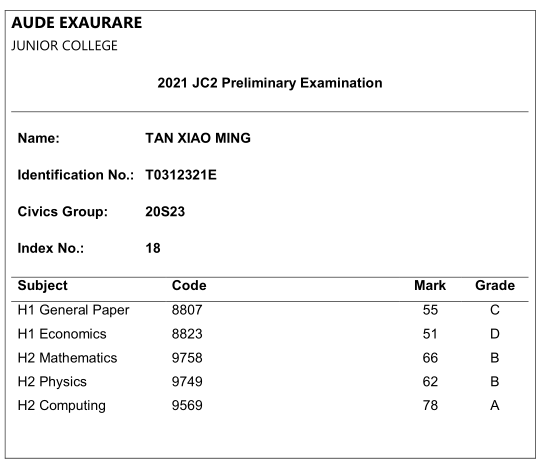
\includegraphics[scale=0.5]{C:/Users/Admin/Desktop/Github/question_bank/LyX/static/img/9569-YIJC-2021-P1-Q4}
\par\end{center}

The college wishes to manage this result information using a relational
database. The normalised database design requires to have a number
of tables. 
\begin{enumerate}
\item Draw an Entity-Relationship (E-R) diagram showing these tables and
the relationships between them. \hfill{}{[}4{]}
\item A table description can be expressed as: 

\texttt{TableName (}\texttt{\uline{Attribute1}}\texttt{, Attribute2{*},
Attribute3, \dots ) }

The primary key is indicated by underlining one or more attributes.
Foreign keys are indicated by using a dashed underline/asterisk. Write
table descriptions for the tables you identified in \textbf{part (a)}.
\hfill{} {[}5{]}
\item Under the Personal Data Protection Act (PDPA), the NRIC/FIN can no
longer be used as a unique identifier for each student. Suggest and
justify a suitable alternative unique identifier for each student.
\hfill{}{[}2{]}
\item Write an SQL query to output the names, civics groups and grades of
students who have obtained at least 60 marks for H2 Computing. \hfill{}{[}4{]}
\end{enumerate}